% Copyright (C) 2005-2015 Airbus - EDF - IMACS - Phimeca
% Permission is granted to copy, distribute and/or modify this document
% under the terms of the GNU Free Documentation License, Version 1.2
% or any later version published by the Free Software Foundation;
% with no Invariant Sections, no Front-Cover Texts, and no Back-Cover
% Texts.  A copy of the license is included in the section entitled "GNU
% Free Documentation License".
\renewcommand{\filename}{docUC_LSF_NMFManipulation.tex}
\renewcommand{\filetitle}{UC : Manipulation of a NumericalMathFunction}

% \HeaderNNIILevel
% \HeaderIILevel
\HeaderIIILevel



\index{Numerical Math Function Manipulation!Dimension}
\index{Numerical Math Function Manipulation!Gradient}
\index{Numerical Math Function Manipulation!Hessian}
\index{Numerical Math Function Manipulation!Marginal}
\index{Numerical Math Function Manipulation!Evaluation}
\index{Numerical Math Function Manipulation!Composition}
\index{Numerical Math Function Manipulation!History}
\index{Numerical Math Function Manipulation!Graph}


The objective of this Use Case  is to describe the main functionalities of OpenTURNS  to manipulate a numerical function $f : \Rset^n  \longrightarrow \Rset^p$.\\

OpenTURNS enables :
\begin{itemize}
\item to ask the dimension of its input and output vectors, with the methods {\itshape getInputDimension,  getOutputDimension},
\item to evaluate itself, its gradient and hessian, with the methods {\itshape gradient, hessian}. The evaluation of the function is a vector of dimension $p$, the gradient is a matrix with $p$ rows and $n$ columns, the hessian is a tensor of order 3 with  $p$ rows, $n$ columns and $n$ sheets,
\item to set a finite difference method for the evaluation of the gradient or the hessian, with the methods {\itshape setGradientImplementation, setHessianImplementation},
\item to evaluate the number of times the function or its gradient or its hessian have been evaluated {\bf since the beginning of the python session}, with the methods {\itshape getEvaluationCallsNumber, getGradientCallsNumber, getHessianCallsNumber},
\item to desable or enable (enabled by default) the history
  mechanism  with the methods   {\itshape disableHistory, enableHistory},
\item to get all the values evaluated by the function and the
  associated inputs with the methods
  {\itshape getInputHistory,  getOutputHistory}
\item to clear the history {\itshape clearHistory},
\item to ask the description of its input and output vectors, with the methods {\itshape getInputDescription,  getOutputDescription},
\item to extract its components if $p>1$, which are functions $f_i : \Rset^n  \longrightarrow \Rset$, with the method {\itshape getMarginal},
\item to ask for its parameters with the method {\itshape getParameters},
\item to define its parameters, with the method {\itshape setParameters},
\item to compose two functions,
\item to ask for the valid operators in OpenTURNS, the valid constants and functions, with the methods {\itshape GetValidOperators, GetValidConstants, GetValidFunctions}.
\end{itemize}

Furthermore,  OpenTURNS implemented an history mechanism to all the NumericalMathFunction types. It is desactivated by default, and stores all the input and output values of a function when activated thanks to the method  {\itshape enableHistory}.\\

It is also possible to draw function graphs, for any function : $f : \mathbb{R}^n \rightarrow \mathbb{R}^p$ where we note $\vect{x} = (x_1, \dots, x_n)$ and $f(\vect{x}) = (f_1(\vect{x}), \dots,f_p(\vect{x}))$, with $n\geq 1$ and $p\geq 1$. OpenTURNS allows to :
\begin{itemize}
\item the graph of any marginal $f_k: \mathbb{R}^n \rightarrow \mathbb{R}$ with respect to the variation of $x_j$ in the intervall $[x_j^{min}, x_j^{max}]$, when all the other components of $\vect{x}$ are fixed to the corresponding ones of the \emph{central point} noted $\vect{CP}$. Then OpenTURNS draws the graph : $t\in [x_j^{min}, x_j^{max}] \mapsto f_k(CP_1, \dots, CP_{j-1}, t,  CP_{j+1} \dots, CP_n)$. The method is $draw(arguments)$ whith the appropriate arguments.
\item the iso-curves of the  function $f_k$ with respect to the variation of $(x_i, x_j)$ in the intervall $[x_i^{min}, x_i^{max}] \times [x_j^{min}, x_j^{max}] $, when all the other components of $\vect{x}$ are fixed to the corresponding ones of the \emph{central point} noted $\vect{CP}$. Then OpenTURNS draws the graph : $(t,u) \in [x_i^{min}, x_i^{max}] \times [x_j^{min}, x_j^{max}] \mapsto f_k(CP_1, \dots, CP_{i-1}, t,  CP_{i+1}, \dots, CP_{j-1}, u,  CP_{j+1} \dots, CP_n)$.
\end{itemize}
The number of points to draw the curve can be specified.\\
There is a simplified call to the metho when $n=p=1$ or when $n=2$ and $p=1$.




\requirements{
  \begin{description}
  \item[$\bullet$] some functions $\Rset^n  \longrightarrow \Rset^p$: {\itshape myFunction, func1, func2, func3, g} (for more details, see above)
  \item[type:] NumericalMathFunction
  \end{description}
}
             {
               \begin{description}
               \item[$\bullet$] none
               \end{description}
             }

             \textspace\\
             Functions used in the script have the following features :
             \begin{itemize}
             \item $myFunction : \mathbb{R}^2 \rightarrow \mathbb{R}^2$ ,
             \item $func1 : \mathbb{R} \rightarrow \mathbb{R}$ ,
             \item $func2 : \mathbb{R}^2 \rightarrow \mathbb{R}$ ,
             \item $func3 : \mathbb{R}^3 \rightarrow \mathbb{R}^2$
             \item $g : \mathbb{R}^2 \rightarrow \mathbb{R}^2$.
             \end{itemize}

             Python script for this Use Case :

             \inputscript{script_docUC_LSF_NMFManipulation}

             Here are the graphs drawn by the script for the functions :
             \begin{itemize}
             \item $func1 : \mathbb{R} \rightarrow \mathbb{R}$ such that $func1(x)  = x^2$ ,
             \item $func2 : \mathbb{R}^2 \rightarrow \mathbb{R}$ such that $func2(x,y)  = xy$ ,
             \item $func3 : \mathbb{R}^3 \rightarrow \mathbb{R}^3$ such that $func3(x,y,z)  =(1+2x+y+z^3, 2+sin(x+2y)-z^4sin(z))$.
             \end{itemize}


             \begin{figure}[H]
               \begin{minipage}{8cm}
                 \begin{center}
                   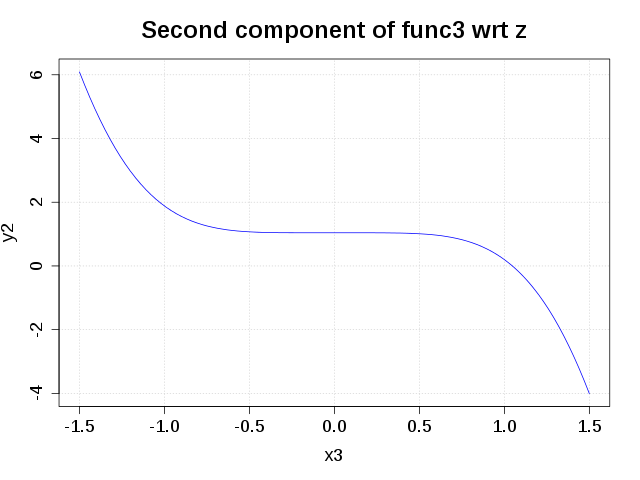
\includegraphics[width=7cm]{Figures/NMFgraph1.png}
                   \caption{Graph of : $ z \mapsto  func3_2(x_0,y_0,z)$, with $(x_0,y_0) = (1.0, 2.0)$ and $z\in [-1.5, 1.5]$.}
                   \label{graph1}
                 \end{center}
               \end{minipage}
               \hfill
               \begin{minipage}{8cm}
                 \begin{center}
                   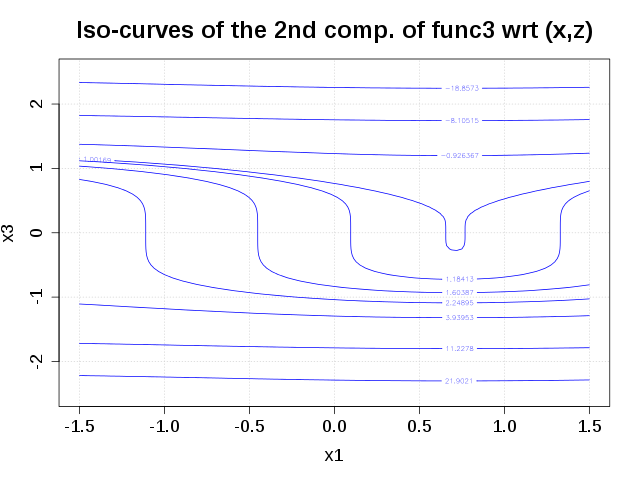
\includegraphics[width=7cm]{Figures/NMFgraph2.png}
                   \caption{Iso-curves of : $ (x,z) \mapsto  func3_2(x_0,y,z)$, with $y_0 = 2.0$ and $x\in [-1.5, 1.5]$ and $z\in [-2.5, 2.5]$.}
                   \label{graph2}
                 \end{center}
               \end{minipage}
             \end{figure}


             \begin{figure}[H]
               \begin{minipage}{8cm}
                 \begin{center}
                   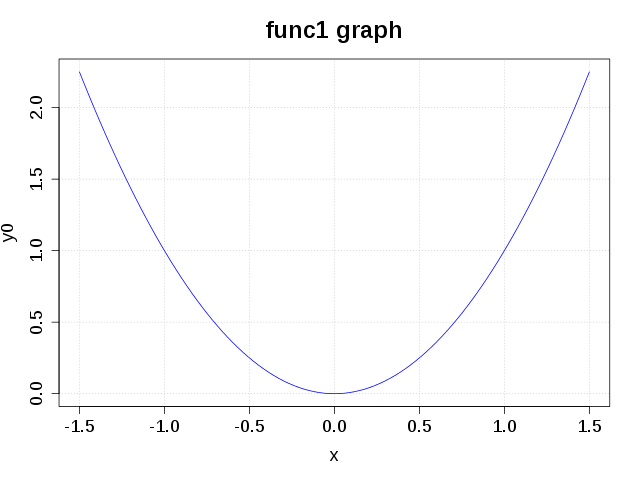
\includegraphics[width=7cm]{Figures/NMFgraph3.png}
                   \caption{Graph of : $ x \mapsto  func1(x)$, with $x\in [-1.5, 1.5]$.}
                   \label{graph1}
                 \end{center}
               \end{minipage}
               \hfill
               \begin{minipage}{8cm}
                 \begin{center}
                   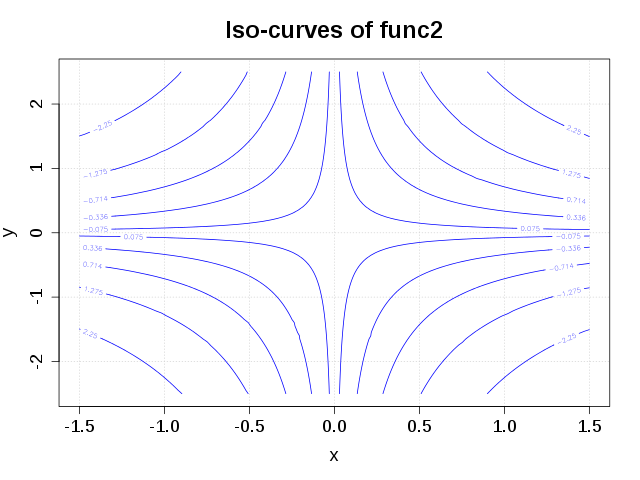
\includegraphics[width=7cm]{Figures/NMFgraph4.png}
                   \caption{Iso-curves of : $ (x,y) \mapsto  func2(x,y)$, with  $x\in [-1.5, 1.5]$ and $y\in [-2.5, 2.5]$.}
                   \label{graph2}
                 \end{center}
               \end{minipage}
             \end{figure}
